%!Tex Root = ../main.tex
% ./Packete.tex
% ./Design.tex
% ./Deklarationen.tex
% ./Vorbereitung.tex
% ./Aufgabe1.tex
% ./Aufgabe2.tex
% ./Aufgabe3.tex
% ./Aufgabe4.tex

\section{Appendix}

\setcounter{exercise}{1}

\begin{frame}[allowframebreaks]{Aufgabe \thesection}{Primimplikantentafel, 1te Regel}
  \begin{itemize}
    \item da es nur darum geht, dass alle Minterme vom Anfang abgedeckt sind und die wesentlichen Minterme auf jeden Fall genommen werden müssen, werden auch die Minterme, die sie abdecken auf jeden Fall genommen. Aus diesem Grund ist es nicht mehr notwendig diese Minterme in der Primimplikantentafel miteinzubeziehen, da man Minterme nur in der Primimplikantentafel miteinbezieht, wenn man noch eine Abdeckung für diese Minterme sucht.
  \end{itemize}
\end{frame}

\begin{frame}[allowframebreaks]{Aufgabe \thesection}{Primimplikantentafel, 2te Regel}
  \begin{columns}
    \begin{column}{0.5\textwidth}
      \begin{table}
      \centering
        \begin{tblr}{
            cells={c, BoxColor},
            row{4} = {SecondaryColorDimmed},
            row{1} = {PrimaryColor, fg=white},
            cell{2}{1} = {PrimaryColor, fg=white},
            cell{3}{1} = {PrimaryColor, fg=white},
            cell{4}{1} = {PrimaryColor, fg=white},
        }
            & 010 & 100 & \StrikeBeginC{110}{ffirst} \\
          \StrikeBeginR{$ab\overline{c}$}&     &     & \StrikeEndR{1}\\
          \StrikeBeginR{$a\overline{c}$} &     & 1   & \StrikeEndR{1} \\
          $a\overline{c}$  &     & 1   & \StrikeEndC{1}{ffirst}   
        \end{tblr}
      \end{table}
    \end{column}
    \begin{column}{0.5\textwidth}
      \begin{table}
      \centering
      \begin{tblr}{
          cells={c, BoxColor},
          row{4} = {SecondaryColorDimmed},
          row{1} = {PrimaryColor, fg=white},
          cell{2}{1} = {PrimaryColor, fg=white},
          cell{3}{1} = {PrimaryColor, fg=white},
          cell{4}{1} = {PrimaryColor, fg=white},
      }
          & 010 & 100 & \StrikeBeginC{110}{ssecond} \\
        $b\overline{c}$ & 1   &     & 1   \\
        \StrikeBeginR{$a\overline{c}$} &     & 1   & \StrikeEndR{1}   \\
        $a\overline{c}$  &     & 1   & \StrikeEndC{1}{ssecond}   
      \end{tblr}
      \end{table}
    \end{column}
  \end{columns}
  \begin{itemize}
    \item eines der Momome, das den Minterm abdeckt der dominiert wird, wird irgendwann aufgrund weiterer Reduktionen mit der ersten und dritten Reduktionsregel wesentlich und wird dann genommen. Sobald dieses Monom genommen wird ist es aufgrund der Teilmengenbeziehung sicher, dass dieses Monom auch den Minterm der den ersteren Minterm dominiert hat abdeckt. Der zweitere Minterm ist somit nicht mehr von Interesse für die Primimplikantentafel, weil man bereits eine Abdeckung für diesen Minterm gefunden hat und es nur darum geht, dass man alle Minterme vom Anfang abgedeckt hat.
    % \item domierende Spalte raus, es ist zwar weggestrichen, aber nur aus Sichtfeld, aber immer noch da wenn eines der Momome genommen wird, dass diesesn Minterm enthält und eines der Momome muss genommen werden, da dieser Minterm immer gleichzeitig mit einem anderen Minterm vorkommt und aufgrund der ersten Regel muss auf jeden Fall einer dieser Minterme die mit diesem übereinstimmen genomemn werden und es geht nur darum, dass dieser Minterm auf jeden Fall drin sein muss (auf welchem Weg auch immer)
  \end{itemize}
\end{frame}

\begin{frame}[allowframebreaks]{Aufgabe \thesection}{Primimplikantentafel, 3te Regel}
  \begin{itemize}
    \item Wenn die On-Menge eines Monoms Teilmenge der On-Menge eines anderen Monoms ist, dann nimmt das Monom mit der größeren On-Menge, da größere ON-Menge weniger Literale bedeutet und somit weniger Kosten. Mit einer größeren On-Menge kann man mehr Minterme auf einmal abdecken und es geht nur darum, dass man am Ende alle Minterme vom Anfang irgendwie abgedeckt hat.
  \end{itemize}
\end{frame}

\begin{frame}[allowframebreaks]{Aufgabe \thesection}{Primimplikantentafel am Hypercube}
  \resizebox{\textwidth}{!}{
    \begin{minipage}[t]{16cm}
      \begin{table}
        \centering
        \begin{tblr}{
            vlines, hlines,
            cells={c, white},
            row{2} = {SecondaryColorDimmed},
            row{6} = {SecondaryColorDimmed},
            row{7} = {SecondaryColorDimmed},
            row{1} = {PrimaryColor, fg=white},
            column{1} = {PrimaryColor, fg=white},
          }
            & \StrikeBeginC{0000}{first} & 0001 & 0100 & 0101 & 0110 & 0111 & 1000 & 1010 & 1100 & 1110 & 1111 \\
        0-0- &  1   &   1  &   1  &   1  &      &      &      &      &      &      &      \\
        --00 &  1   &      &   1  &      &      &      &   1  &      &  1   &      &      \\
        01-- &      &      &   1  &   1  & 1    & 1    &      &      &      &      &      \\
        -11- &      &      &   1  &      &   1  &      &      &      &   1  &  1   &      \\
        -1-0 &      &      &      &      &   1  &  1   &      &      &      &  1   &   1  \\
        1--0 &      &      &      &      &      &      &   1  &   1  &   1  &  1   &      \\
        \end{tblr}
      \end{table}
    \end{minipage}
  }
  \pagebreak

  \resizebox{\textwidth}{!}{
    \begin{minipage}[t]{16cm}
      \begin{table}
        \centering
        \begin{tblr}{
            vlines, hlines,
            cells={c, white},
            row{2} = {SecondaryColorDimmed},
            row{6} = {SecondaryColorDimmed},
            row{7} = {SecondaryColorDimmed},
            row{1} = {PrimaryColor, fg=white},
            column{1} = {PrimaryColor, fg=white},
          }
            & \StrikeBeginC{0000}{first} & \StrikeBeginC{0001}{second} & \StrikeBeginC{0100}{third} & \StrikeBeginC{0101}{four} & \StrikeBeginC{0110}{five} & \StrikeBeginC{0111}{six} & \StrikeBeginC{1000}{seven} & \StrikeBeginC{1010}{eight} & \StrikeBeginC{1100}{nine} & \StrikeBeginC{1110}{ten} & \StrikeBeginC{1111}{eleven} \\
        0-0- &  1   &   1  &   1  &   1  &      &      &      &      &      &      &      \\
        --00 &  1   &      &   1  &      &      &      &   1  &      &  1   &      &      \\
        01-- &      &      &   1  &   1  & 1    & 1    &      &      &      &      &      \\
        -11- &      &      &   1  &      &   1  &      &      &      &   1  &  1   &      \\
        -1-0 &      &      &      &      &   1  &  1   &      &      &      &  1   &   1  \\
        1--0 &  \StrikeEndC{}{first}    &  \StrikeEndC{}{second}    & \StrikeEndC{}{third}     &  \StrikeEndC{}{four}    &  \StrikeEndC{}{five}    &  \StrikeEndC{}{six}    &   \StrikeEndC{1}{seven}  &   \StrikeEndC{1}{eight}  &   \StrikeEndC{1}{nine}  &  \StrikeEndC{1}{ten}   &  \StrikeEndC{}{eleven}    \\
        \end{tblr}
      \end{table}
    \end{minipage}
  }
  \begin{itemize}
    \item $(\overline{x_0}\overline{x_2})\vee(x_1\overline{x_3})\vee(x_0\overline{x_3})$, $\{0{-}0{-}, {-}1{-}0 ,1{-}{-}0\}$
  \end{itemize}

  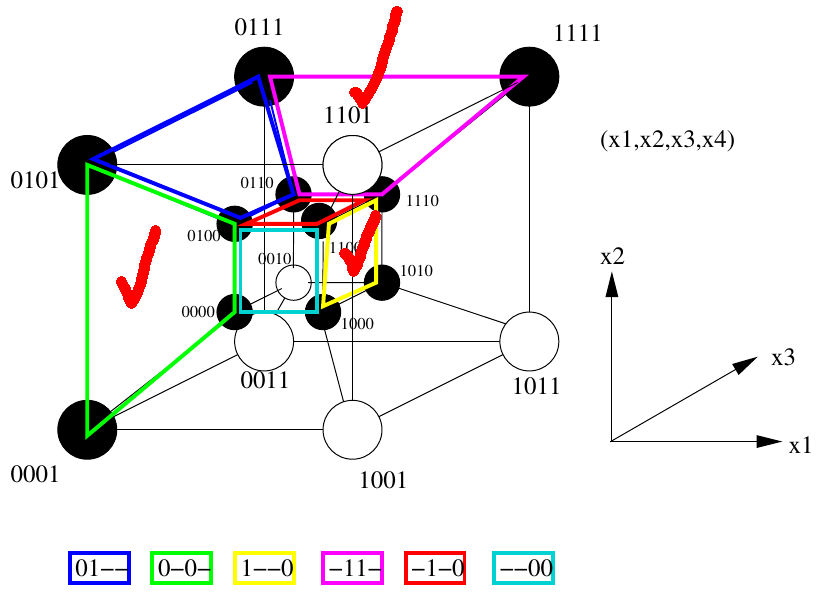
\includegraphics[height=0.6\paperheight, center]{./figures/hypercube.png}
\end{frame}

\begin{frame}[allowframebreaks]{Aufgabe \thesection}{Binärbaum, wobei $n=2^k$}
  \begin{columns}
    \begin{column}{0.6\textwidth}
      \resizebox{\textwidth}{!}{
        \begin{minipage}[t]{8cm}
          \begin{itemize}
            \item \alert{Anzahl Blätter (vollständiger Binärbaum):} $n = 2^d = 2^3 = 8$
            \item \alert{Anzahl Knoten:}  $\displaystyle k = \sum_{i=0}^{d} 2^i = \frac{2^{d+1}-1}{2-1} = 2^{d+1}-1 = 2^{3+1}-1 = 1 + 2 + 4 + 8 = 15$
            \item \alert{Tiefe mithilfe Anzahl Blätter:} $d = log_2(n) = log_2(8) = 3$
            \item \alert{Tiefe mithilfe Anzahl Knoten (vollständiger Baum):} $d = log_2(k + 1) - 1 = log_2(15 + 1) - 1 = 4 - 1 = 3$
            \begin{itemize}
              \item \alert{Herleitung:} $2^{d+1}-1 = k \Leftrightarrow 2^{d+1} = k + 1\Leftrightarrow log_2(2^{d+1}) = log_2(k + 1) \Leftrightarrow d+1 = log_2(k + 1) \Leftrightarrow d = log_2(k + 1) - 1$
            \end{itemize}
            \item  \alert{Tiefe mithilfe Anzahl Knoten:} $d = \lfloor(log_2(k_{real}))\rfloor = \lfloor log_2(10)\rfloor = 3$
            \begin{itemize}
              \item $d = \lfloor(log_2(k_{real}))\rfloor = \lfloor log_2(8)\rfloor = 3$
              \item $d = \lfloor(log_2(k_{real}))\rfloor = \lfloor log_2(7)\rfloor = 2$
            \end{itemize}
          \end{itemize}
        \end{minipage}
      }
    \end{column}
    \begin{column}{0.4\textwidth}
      \resizebox{\textwidth}{!}{
        \begin{minipage}[t]{6cm}
          \ctikzfig{./figures/binary_tree}
        \end{minipage}
      }
    \end{column}
  \end{columns}
\end{frame}
